\documentclass[a4paper]{report}

\usepackage{amsmath}

\title{Vaja 22 Viskoznost}
\author{Jure Kos}
\date{14.10.2021}
\usepackage{graphicx}
\graphicspath{{./images/}}

\begin{document}

\maketitle
\chapter*{Uvod}
V realnih tekočinah se zaradi viskoznosti hitrejše plasti v tekočini vlečejo počasnejše in zadržujejo še hitrejše. Tako nastane v pravokotni smeri gradient hitrosti (strižna hitrost). Med sosednjima plastema deluje strižna sila, ki je sorazmerna velikosti stične ploskve in strižni hitrosti (sprememba hitrosti plasti po spremembi višine). To lahko opišemo z enačbo
\[F = \eta \frac{\Delta v}{\Delta y} S \]
kjer sorazmernostni koeficient \(\eta\) poimenujemo koeficient viskoznosti (enota Pa$\cdot$s).

\section*{Potek vaje}
Uporabili smo koaksialni viskozimeter, ki smo ga za meritev viskoznosti potopili v viskozno tekočino do dveh globin. Na škripec smo obesili uteži s tremi različnimi masami (10g, 20g, 30g) in s fotovrati merili hitrost vrtenja viskozimetra. \\

\noindent Za določitev vztrajnostnega momenta viskozimetra smo viskozimeter zavrteli z utežjo brez da bi ga potopili v tekočino. Za meritev navora trenja pa smo viskozimeter zavrteli z začetno hitrostjo in s pomočjo pojemka kotne hitrosti in vztrajnostnega momenta določili navor trenja. 


\section*{Naloga}
1. Izmeriti koeficient viskoznosti dane tekočine.\\
2. Določiti navor trenja v ležajih koaksialnega viskozimetra.


\section*{Potrebščine}
1. Koaksialni viskozimeter,\\
2. neznana tekočina,\\
3. uteži,\\
4. štoparica,\\
5. vrvica,\\
6. merilnik časovnih intervalov,\\
7. računalnik z merilnim vmesnikom.\\

\chapter*{Meritve}
\section*{Moment in navor trenja}
Izmerjene vrednosti vztrajnostnega momenta:
\[
\begin{array}{|c|c|}\hline
  J [kg m^2] & \Delta J [kgm^2] \\ \hline
  0.00067 &  0.00007\\
  0.00068 &  0.00007\\
  0.00067 &  0.00007\\
  \hline
\end{array}
\]
\[\overline{J} = (0.00067 \pm 0.00007) kgm^2\]
\vspace{70mm}
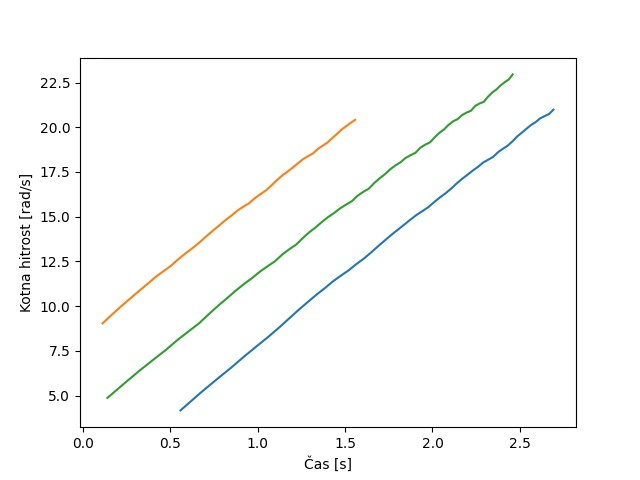
\includegraphics[width=\textwidth]{pospesek}
Izmerjene vrednosti navora trenja:
\[
\begin{array}{|c|c|}\hline
  M_{trenja} [Nm] & \Delta M [Nm] \\ \hline
 -0.00124 &  0.00014\\
 -0.00101 &  0.00012\\
 -0.00085 &  0.00011\\
  \hline
\end{array}
\]
\[\overline{M_{trenja}} = (-0.00103 \pm 0.00011) Nm\]
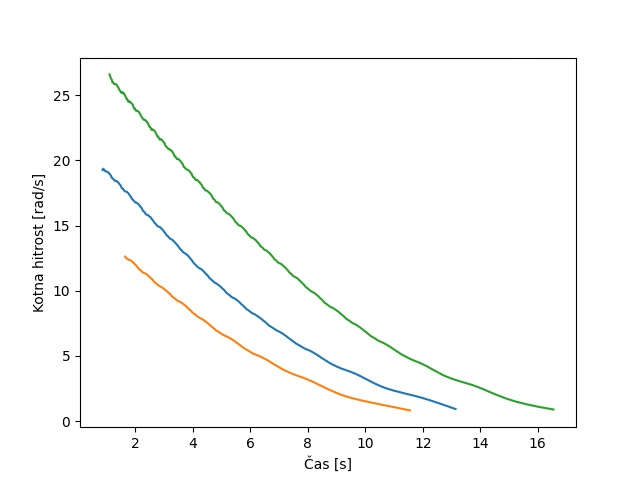
\includegraphics[width=\textwidth]{trenje}

\chapter*{Računi}

\[
\begin{array}{|c|c|}\hline
  \eta [Pa s] & \Delta \eta [Pa s] \\ \hline
  2.4461 &  0.4725\\
  2.1880 &  0.4136\\
  2.2203 &  0.4174\\
  2.0057 &  0.3464\\
  2.3861 &  0.4608\\
  2.2143 &  0.4186\\
  2.2620 &  0.4253\\
  2.4037 &  0.4307\\
  2.0206 &  0.3514\\
  2.0428 &  0.3528\\
  2.2408 &  0.4236\\
  2.2554 &  0.4241\\
  2.2003 &  0.3936\\
  2.0139 &  0.3503\\
  2.0726 &  0.3580\\
  \hline
\end{array}
\]

\noindent Za izračun viskoznosti za posamezen poskus smo uporabili le časovni interval, kjer je bila kotna hitrost v povprečju konstantna. Takrat velja:
\[ \eta = \frac{mgr_{g} - M_{trenja}}{k\omega(\infty)} \]
\noindent Z upoštevanjem vseh poskusov in navora trenja tako dobimo vrednost viskoznosti tekočine. 
\[\overline{\eta} =2.2Pas \pm 0.4Pas\]

\noindent Glede na podatke na internetu izračunana vrednost tekočino uvršča nekam med viskoznost glicerola (1.5) in sirupa za palačinke (2.5), ker se zdi smiselno.



\chapter*{Grafi}
Graf kotne hitrosti ob najmanjši obremenitvi:\\
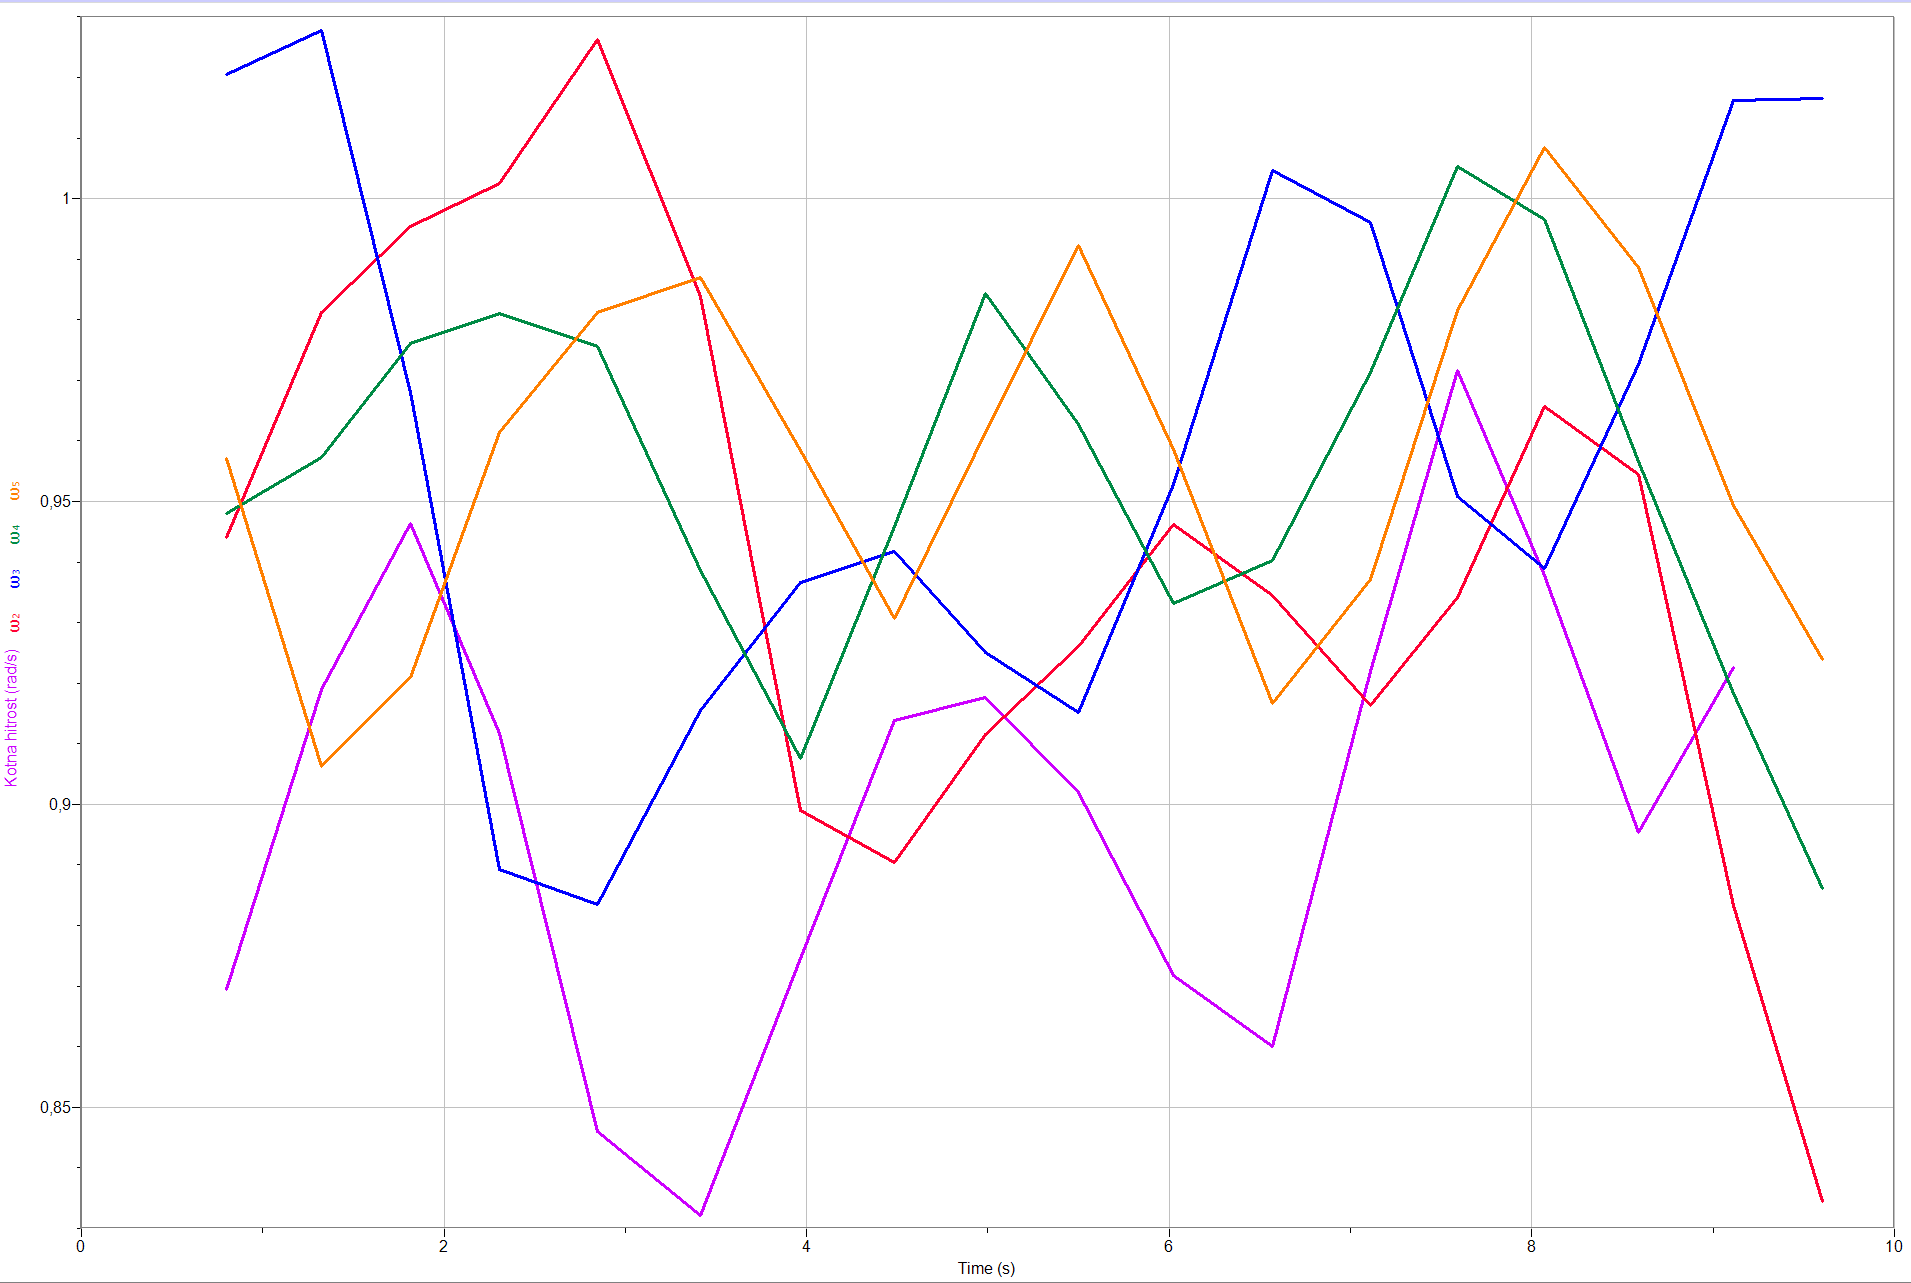
\includegraphics[width=\textwidth]{majhna}\\
\pagebreak

Graf kotne hitrosti ob srednji obremenitvi:\\
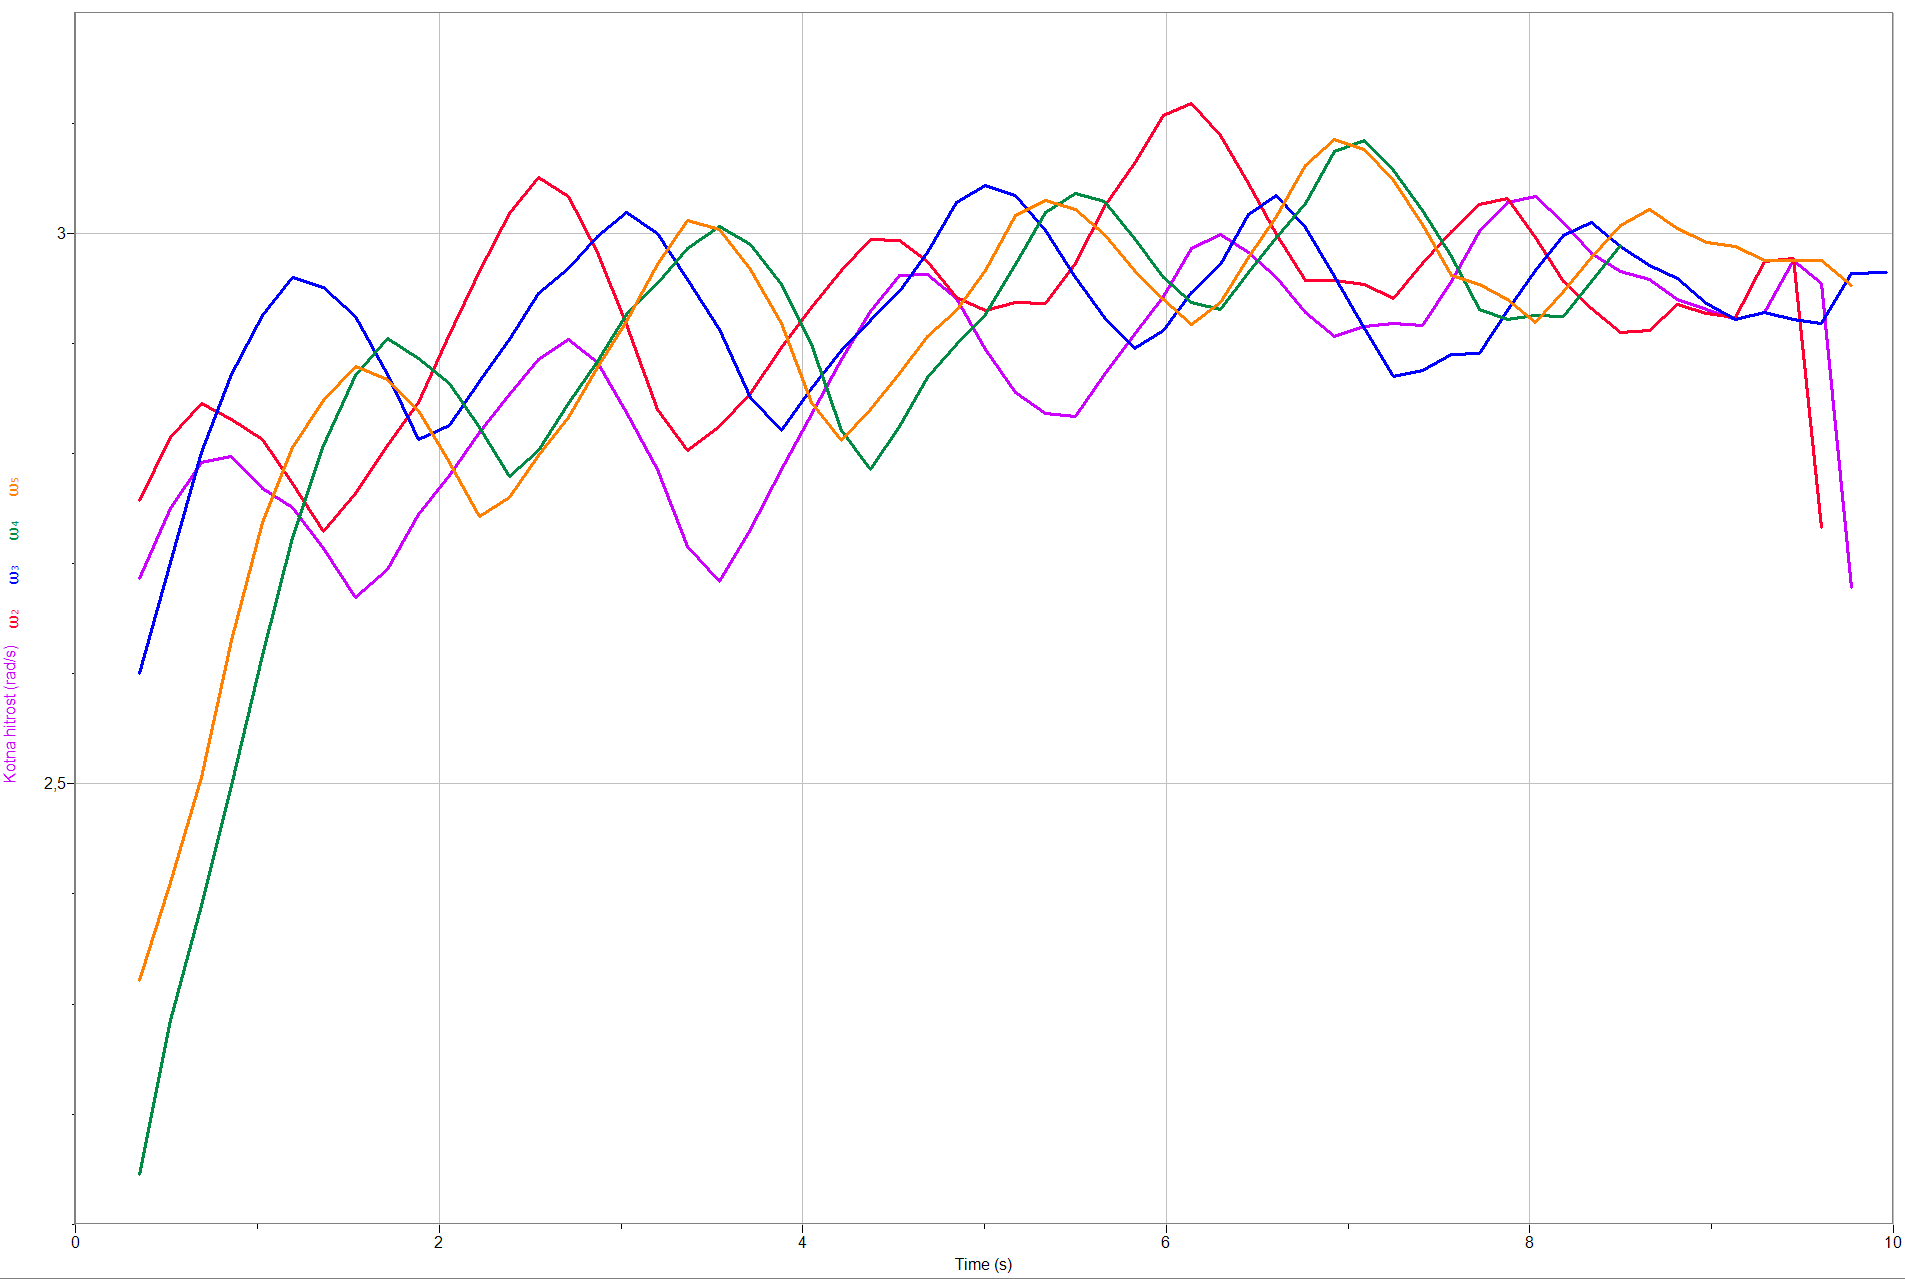
\includegraphics[width=\textwidth]{srednja}\\

Graf kotne hitrosti ob največji obremenitvi:\\
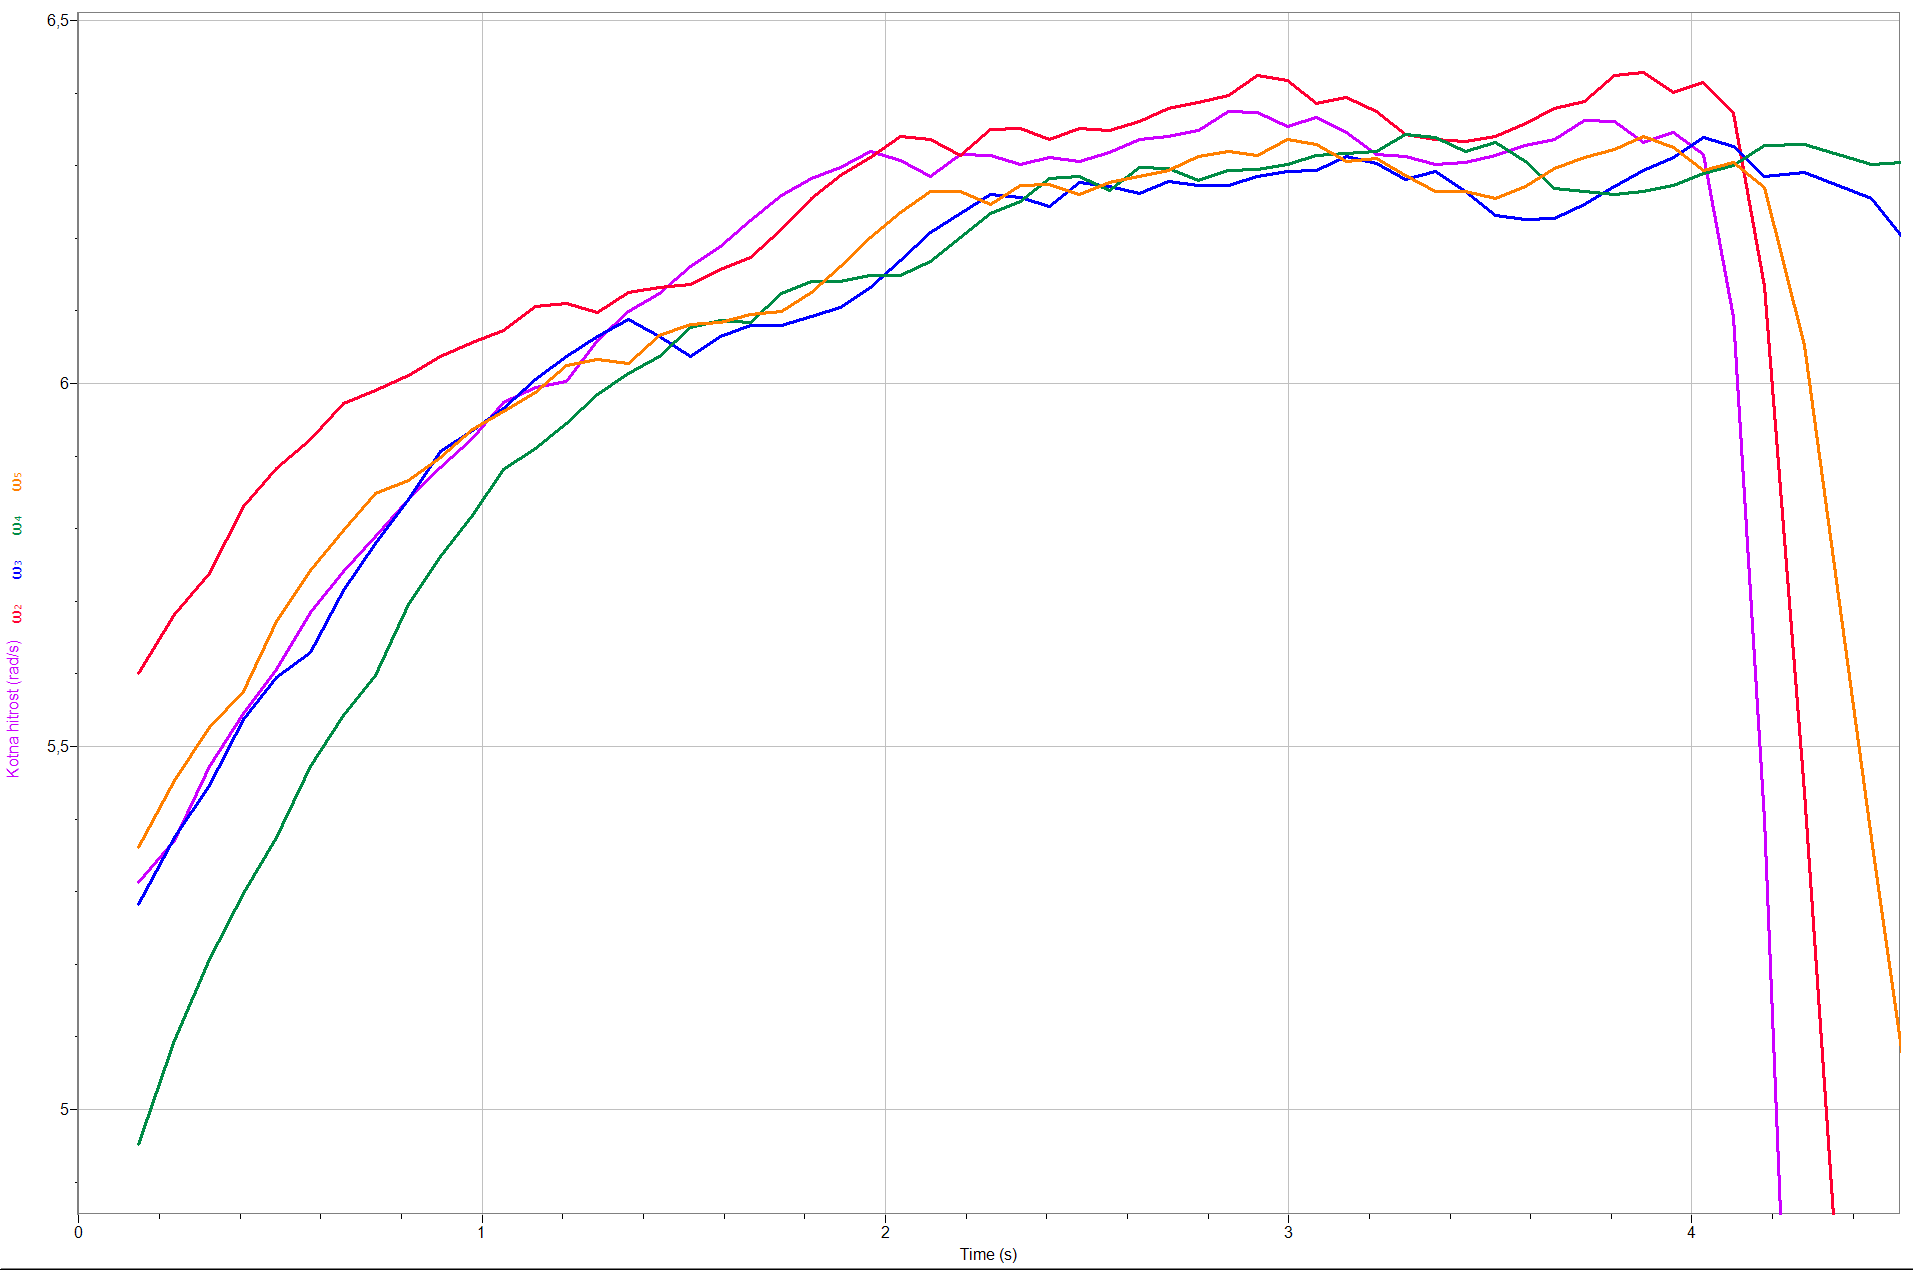
\includegraphics[width=\textwidth]{velika}\\

\end{document}